\part{Sistema solare: pianeti maggiori, asteroidi, anelli e comete. Evoluzione}
\frame{\partpage}

\input{solarsystem}

\part{Formazione dei sistemi planetari}
\frame{\partpage}

\input{formation}

\part{Sistemi extra-solari; pianeti abitabili.}
\frame{\partpage}

\section{extrasolar: todo}

\begin{wordonframe}{Osservazioni: Da ''Physical properties of extrasolar planets''}\tolbf
\begin{itemize}
\item Observed properties: ralation host star metallicity-frequency pf planets, large radius of transiting planets; pg 42 radius anomaly, brown dwarf vs massive planets, Hot Neptune (link to seminario?), light from exoplanets.
\item Interior structure: pg13 EOS composition, Earth-super Earth and Neptune-Super jupiter (18-19); Evolution (pg 30)
\end{itemize}
\end{wordonframe}

\begin{wordonframe}{Udry 03:I, II}
constrain on migration scenario: runaway migration
\end{wordonframe}

\section{Osservazioni}

\begin{wordonframe}{extrasolar: problemi aperti}
Distinzione pianeta/brown dwarf: $M_P\leq20M_J$, i pianeti veri e propri hanno masse $M_P\leq13M_J$.
Domande fondamentali:
\begin{itemize}
    \item Quanto \'e frequente la formazione di sistemi planetari all'atto di formazione stellare?
    \item Quanto \'e frequente la formazione di pianeti terrestri?
    \item Quanto \'e frequente la nascita della vita?
\end{itemize}
\end{wordonframe}

\begin{frame}[allowframebreaks]{Survey}
\begin{columns}[T]\begin{column}{0.5\textwidth}
\begin{block}{RV}
\begin{itemize}
\item Keck: Cumming 08 ($P<2000d$, $m>0.3\mjupiter$) - Keck and Lick: Howard 10
\item California planet survey (exoplanets.org)
\item HARPS (mayor 11)
\end{itemize}
\end{block}
\end{column}\begin{column}{0.5\textwidth}
\begin{itemize}
\item Corot (Moutou 13)
\item Kepler (kelper-california survey II, III, V, planet occurrence within 0.25 AU, taloe of evaporation): Coughlin 16
\end{itemize}
\end{column}\end{columns}
\begin{itemize}
\item Direct imaging: Bowler 16.
\item Microlensing: cassan 12
\end{itemize}
\begin{block}{Exoplanets catalog}
\begin{itemize}
\item Extrasolar planet encyclopedia: exoplanet.eu
\item Keck, lick, Anglo-Australian telescope: exoplanets.org
\item www.inscience.ch/transits: transit references
nsted.ipac.caltech.edu: nasa planet finding and characterization activities 
\end{itemize}
\end{block}
\end{frame}

\section{Properties of radial velocity exoplanets}
%
\begin{wordonframe}{Revs about stat properties of rv exo}
Udry 03, Udry Santos 07, Santos 08, Johnson 09, Mayor 11 Winn Fabrycky 15, Cumming 14
\end{wordonframe}

\begin{frame}{Fraction of stars with orbiting planets. Detectability in M-P diagram.}

\begin{figure}[!ht]
\begin{subfigure}[b]{0.47\textwidth}
\centering
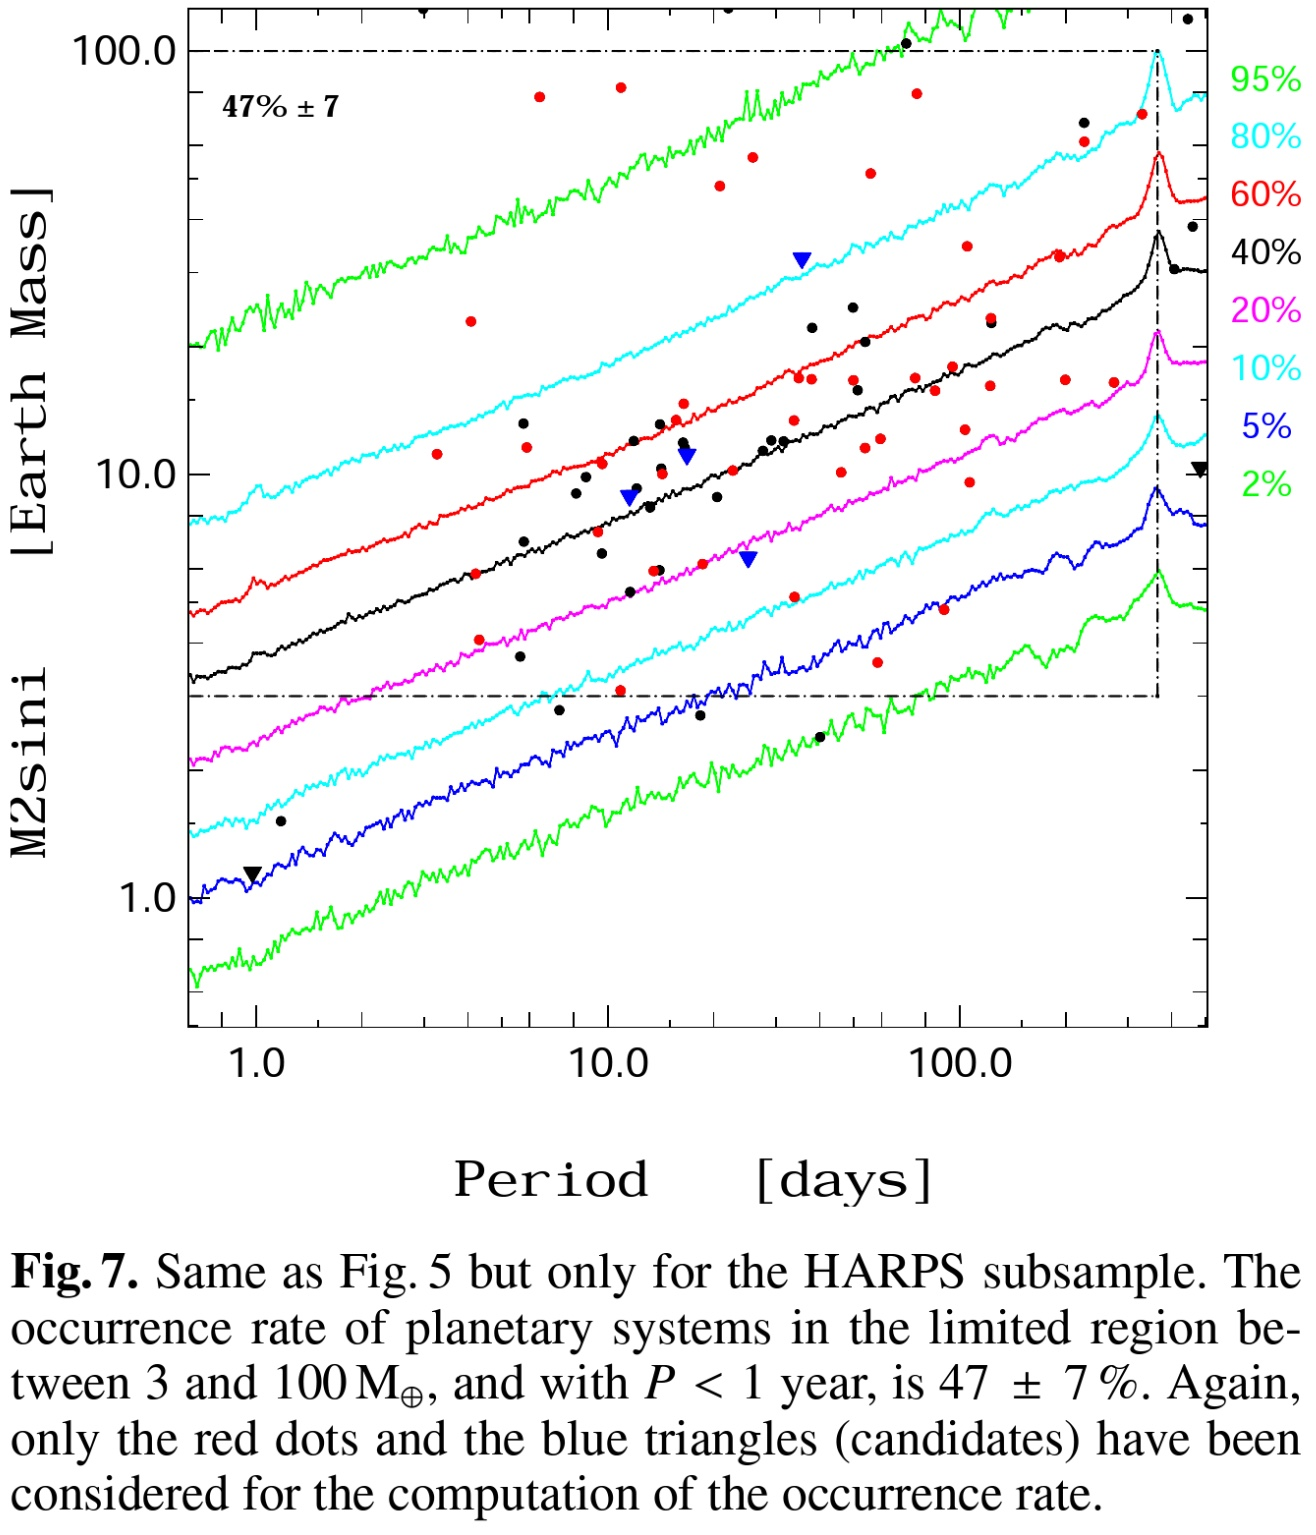
\includegraphics[trim={0cm 0 1 0},clip, keepaspectratio, height=0.4\textheight]{PMfreq-e12}
\label{fig:PMfreq-e12}
\end{subfigure} 
~
\begin{subfigure}[b]{0.47\textwidth}
\centering
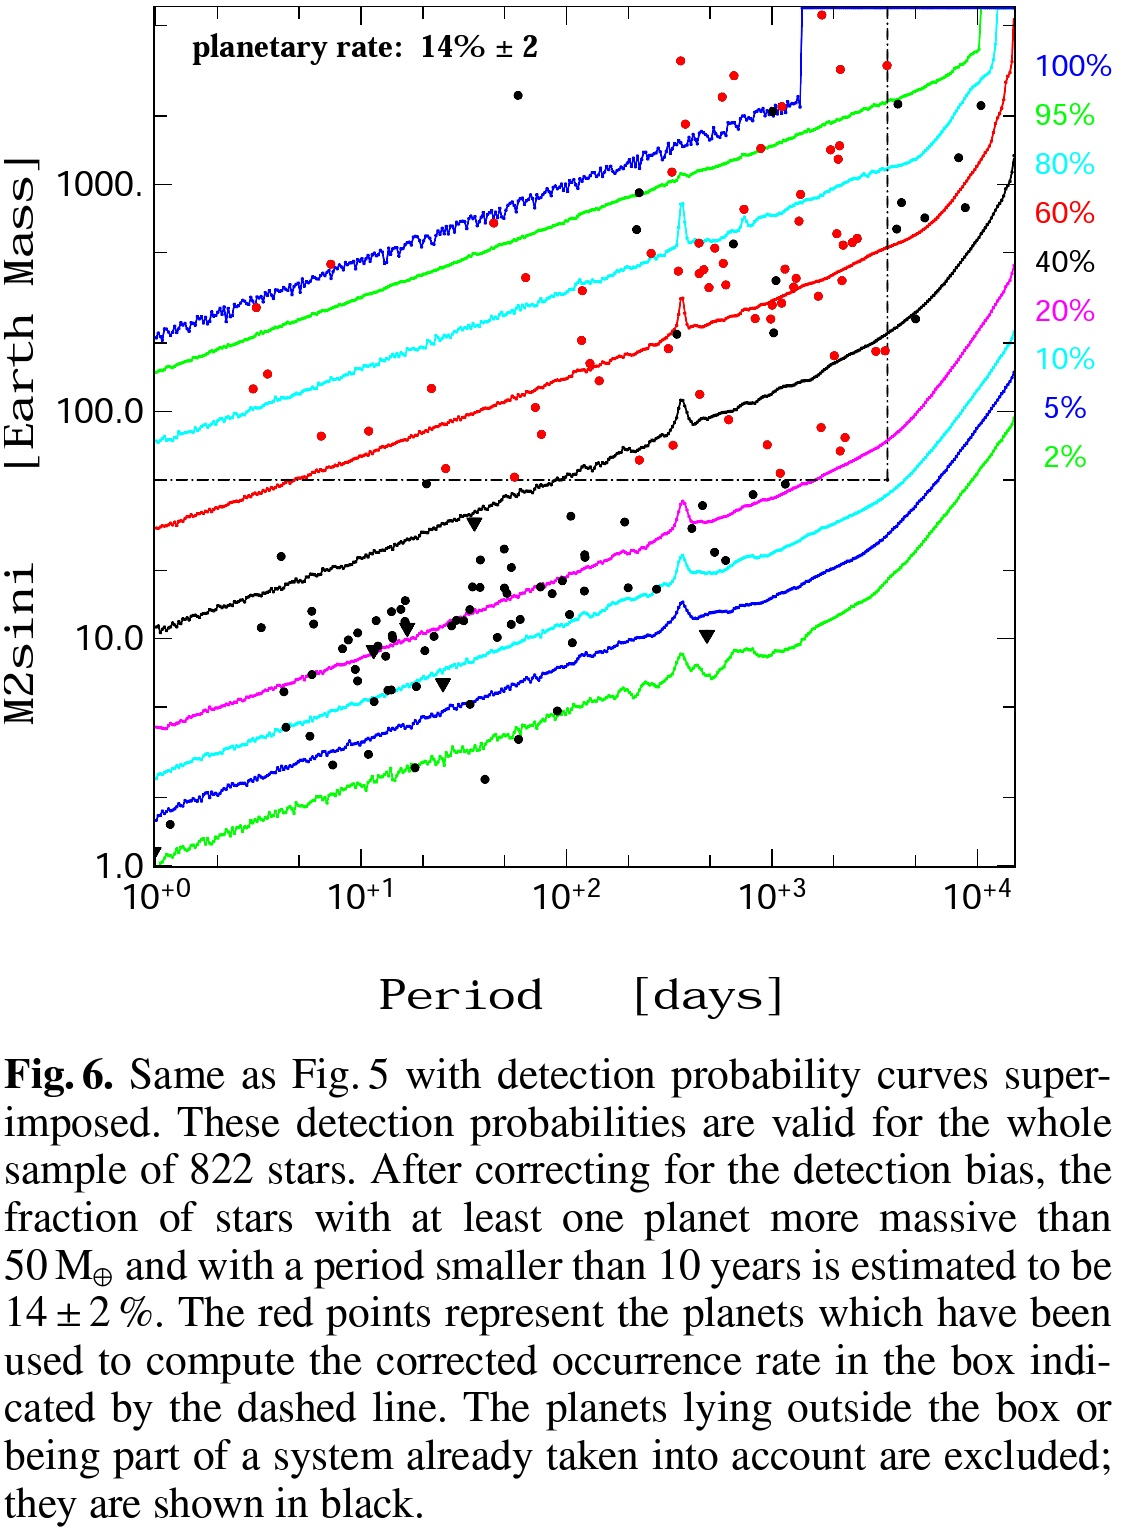
\includegraphics[trim={0cm 0 1 0},clip, keepaspectratio, height=0.4\textheight]{PMfreq-e23}
\label{fig:PMfreq-e23}
\end{subfigure}

\end{figure} 

\begin{figure}[!ht]
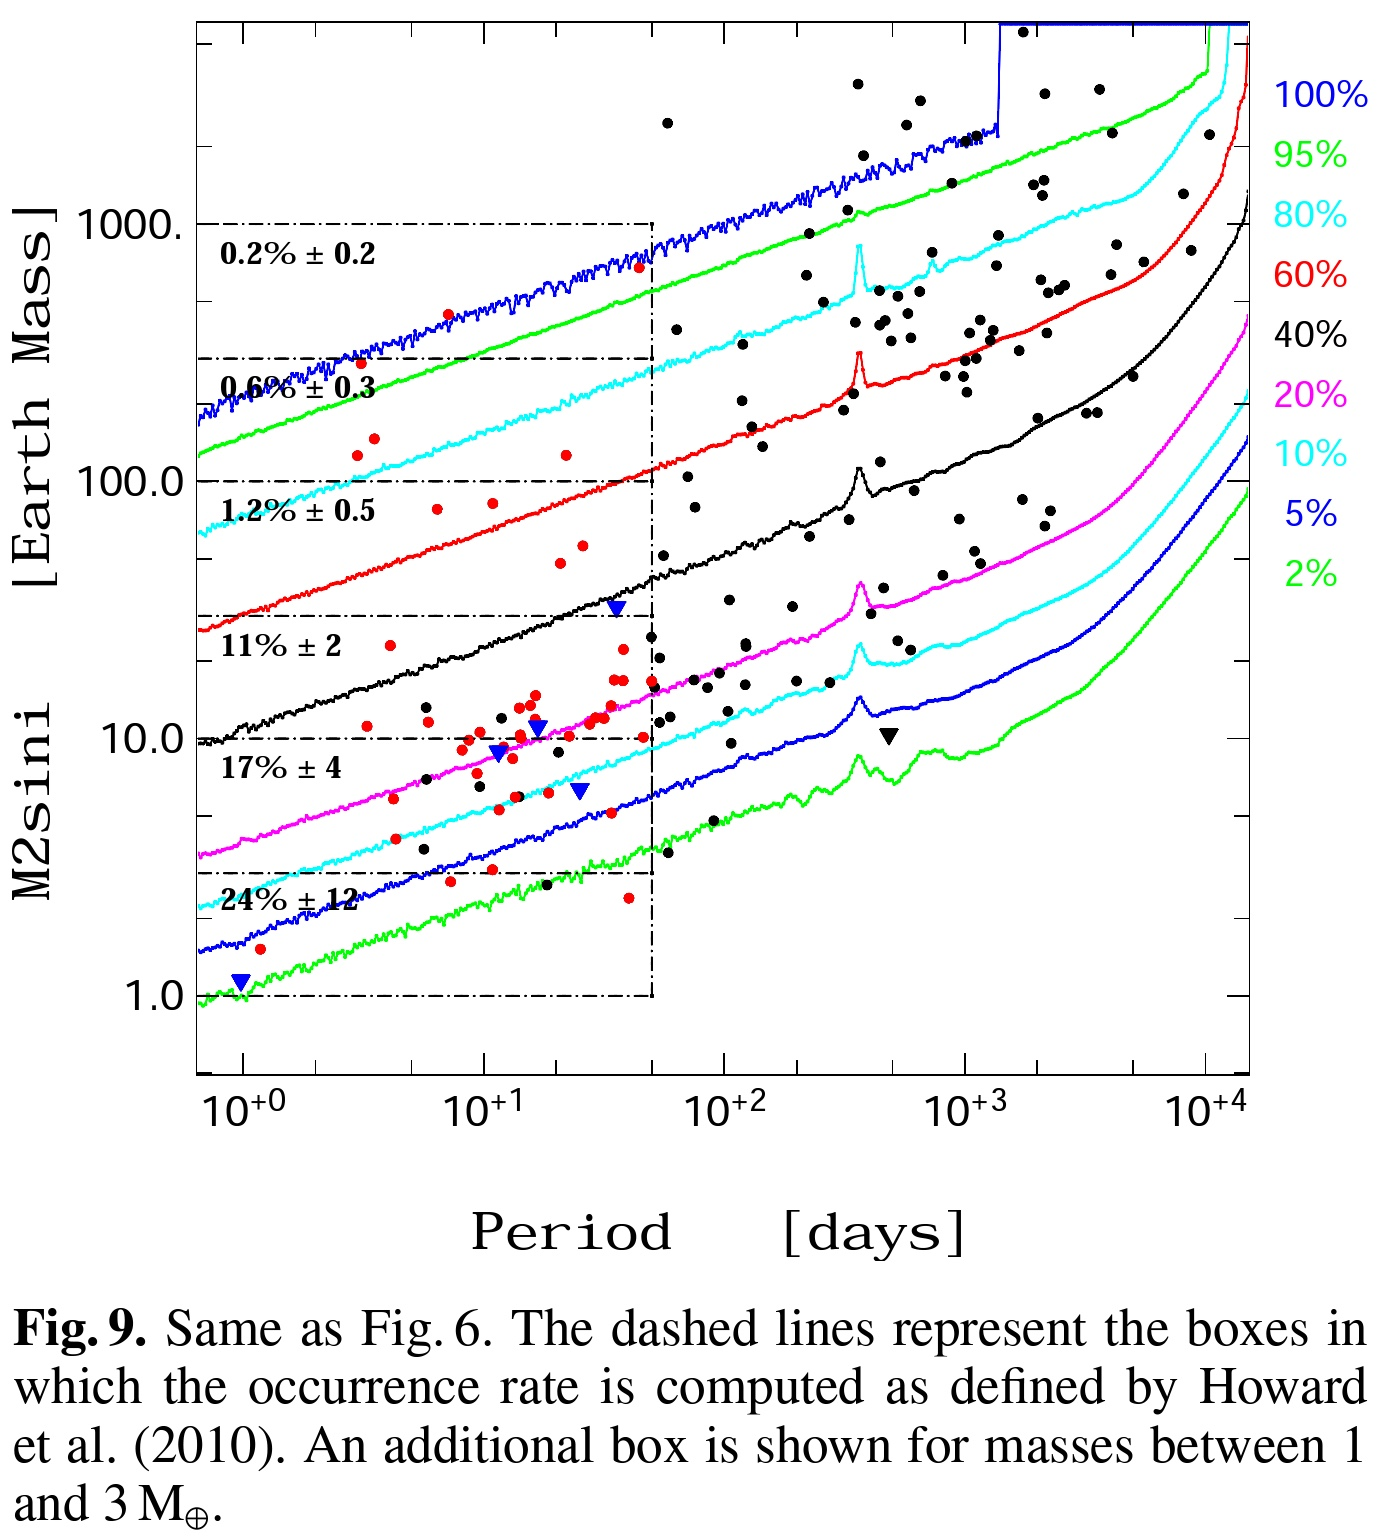
\includegraphics[trim={0cm 0cm 1 0},clip, keepaspectratio,height=0.4\textheight]{PMfreqshort}
\label{fig:PMfreqshort}
\end{figure}

\end{frame}

\begin{wordonframe}{Distribuzioni pianeti osservati tramite RV e completezza survey nello spazio dei parametri M-P}
Le linee colorate nel diagramma massa-periodo delimitano regioni al di sotto delle quali la percentuale indicata ($C(M\sin{i},P)$) di stelle ha $99\%$ di probabilit\'a di rilevamento per un pianeta in quella regione del diagramma.
Il $47\%$ di stelle ospita un pianeta nel range di massa $2\mearth{}-50\mearth{}$ delle super-terre e pianeti gioviani entro $100\mearth{}$, il $14\%$ ha pianeti gioviani ($M_p>50\mearth{}$), il $24\%$, $17\%$ e $11\%$ risp. hanno pianeta terrestre, super-terra e nettuniano con periodo entro $50d$.

$f_{pl}=\frac{1}{N_*}\sum_iN_{ij}$, $N_{ij}=\frac{1}{C(m\sin{i},P)}$ per pianeta i attorno a stella j.
\end{wordonframe}

\begin{frame}{Mass-Period distribution}
\begin{itemize}
\item \cite{marcy2008exoplanet}: Pianeti nel range di massa $0.1-12\mjupiter$ hanno distribuzione di massa $\TDy{M}{N}\propto M\expy{-1.15}$.
\item \cite{cumming2008keck}: nell'intervallo $M=0.3-10\mjupiter{}$ e $P=2-2000\si{\day}$ la distribuzione dei pianeti nel diagramma M-P segue $dn\propto M\expy{\alpha}P\expy{\beta}\,d\log{M}d\log{P}$ con $\alpha=-0.31\pm0.2$, $\beta=0.26\pm0.1$.
\item \cite{mayor2011harps}: $P<\SI{100}{d}$ dominano super-terre e pianeti nettuniani, shortage of massive planets at short periods ($0.5-1\%$ Hot Jupiters), frequency of gaseus giant planets strongly increasing with $\log{P}$, lack of light planet ($M<0.75\mjupiter{}$) on periods larger than \SI{100}{day}.
\end{itemize}
\end{frame}

\begin{frame}{Distribuzione di massa planetaria: RV, Mayor 11}
\begin{figure}[!ht] \begin{subfigure}[b]{0.47\textwidth}
\centering 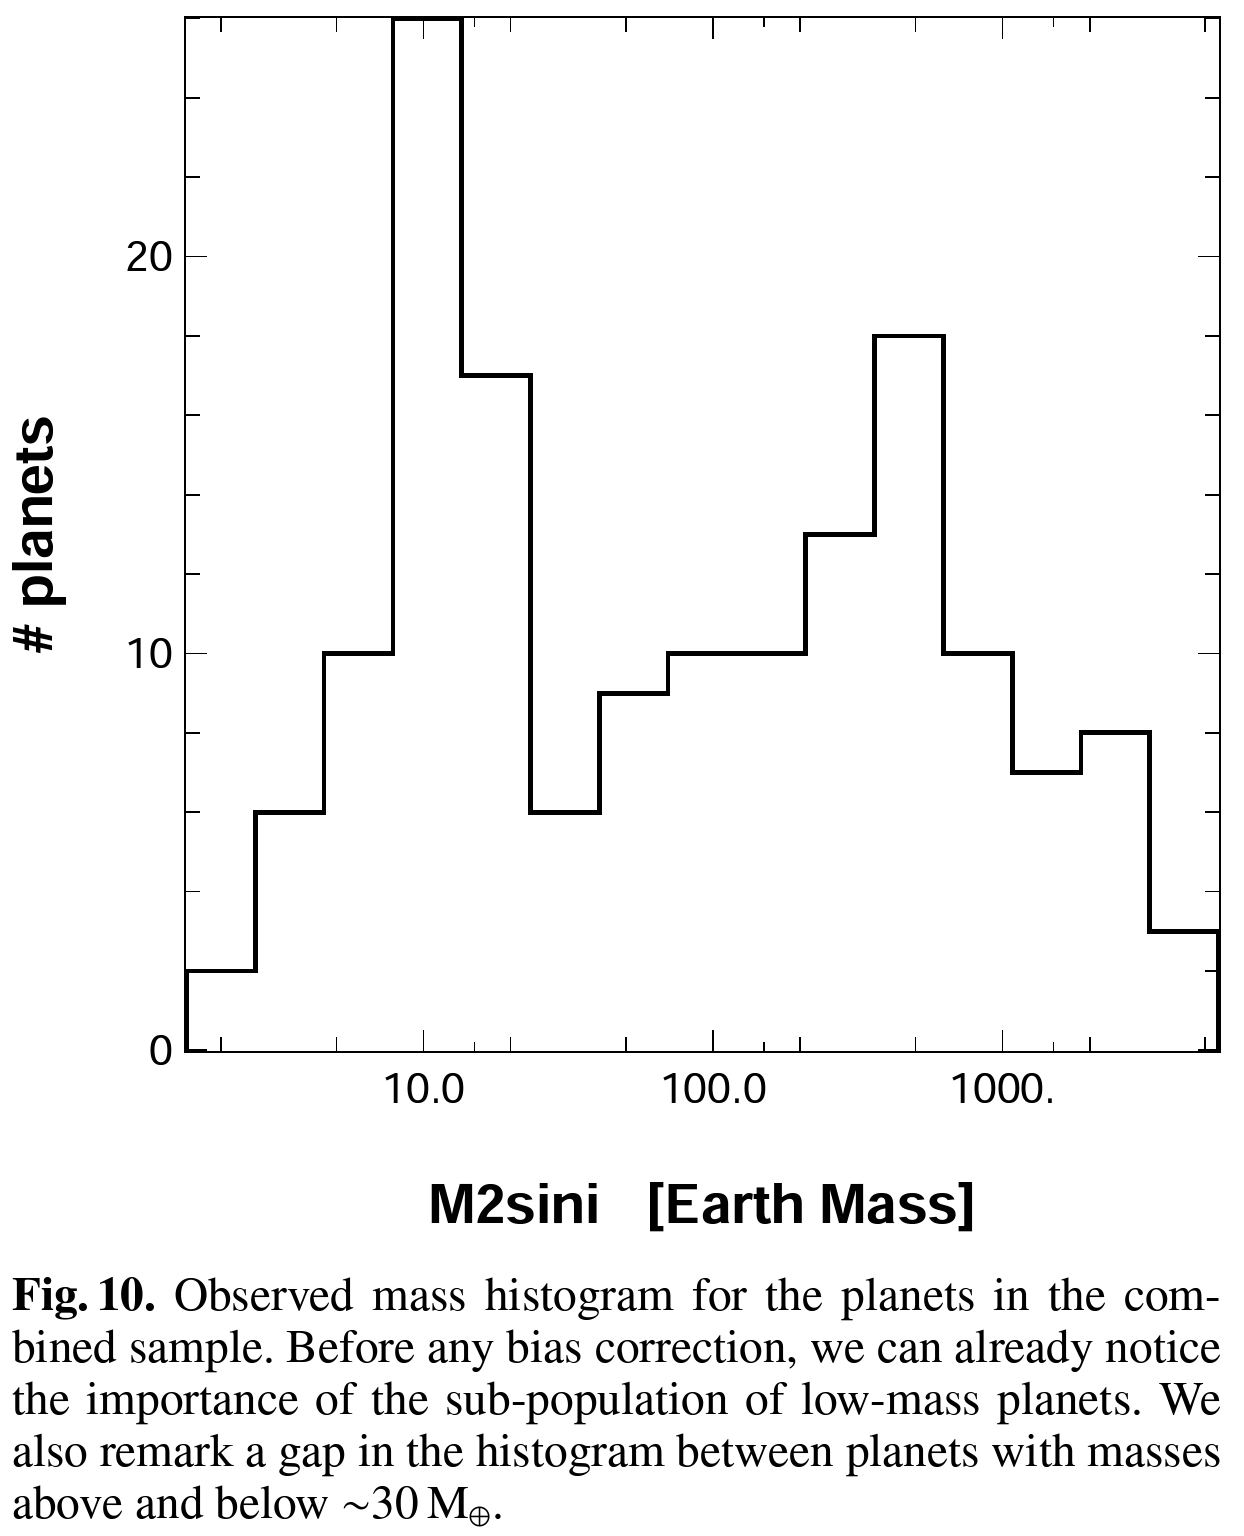
\includegraphics[trim={0cm 0 0 0},clip, height=0.45\textheight]{pvsM} \label{fig:pvsM} \end{subfigure}
~
\begin{subfigure}[b]{0.47\textwidth} \centering 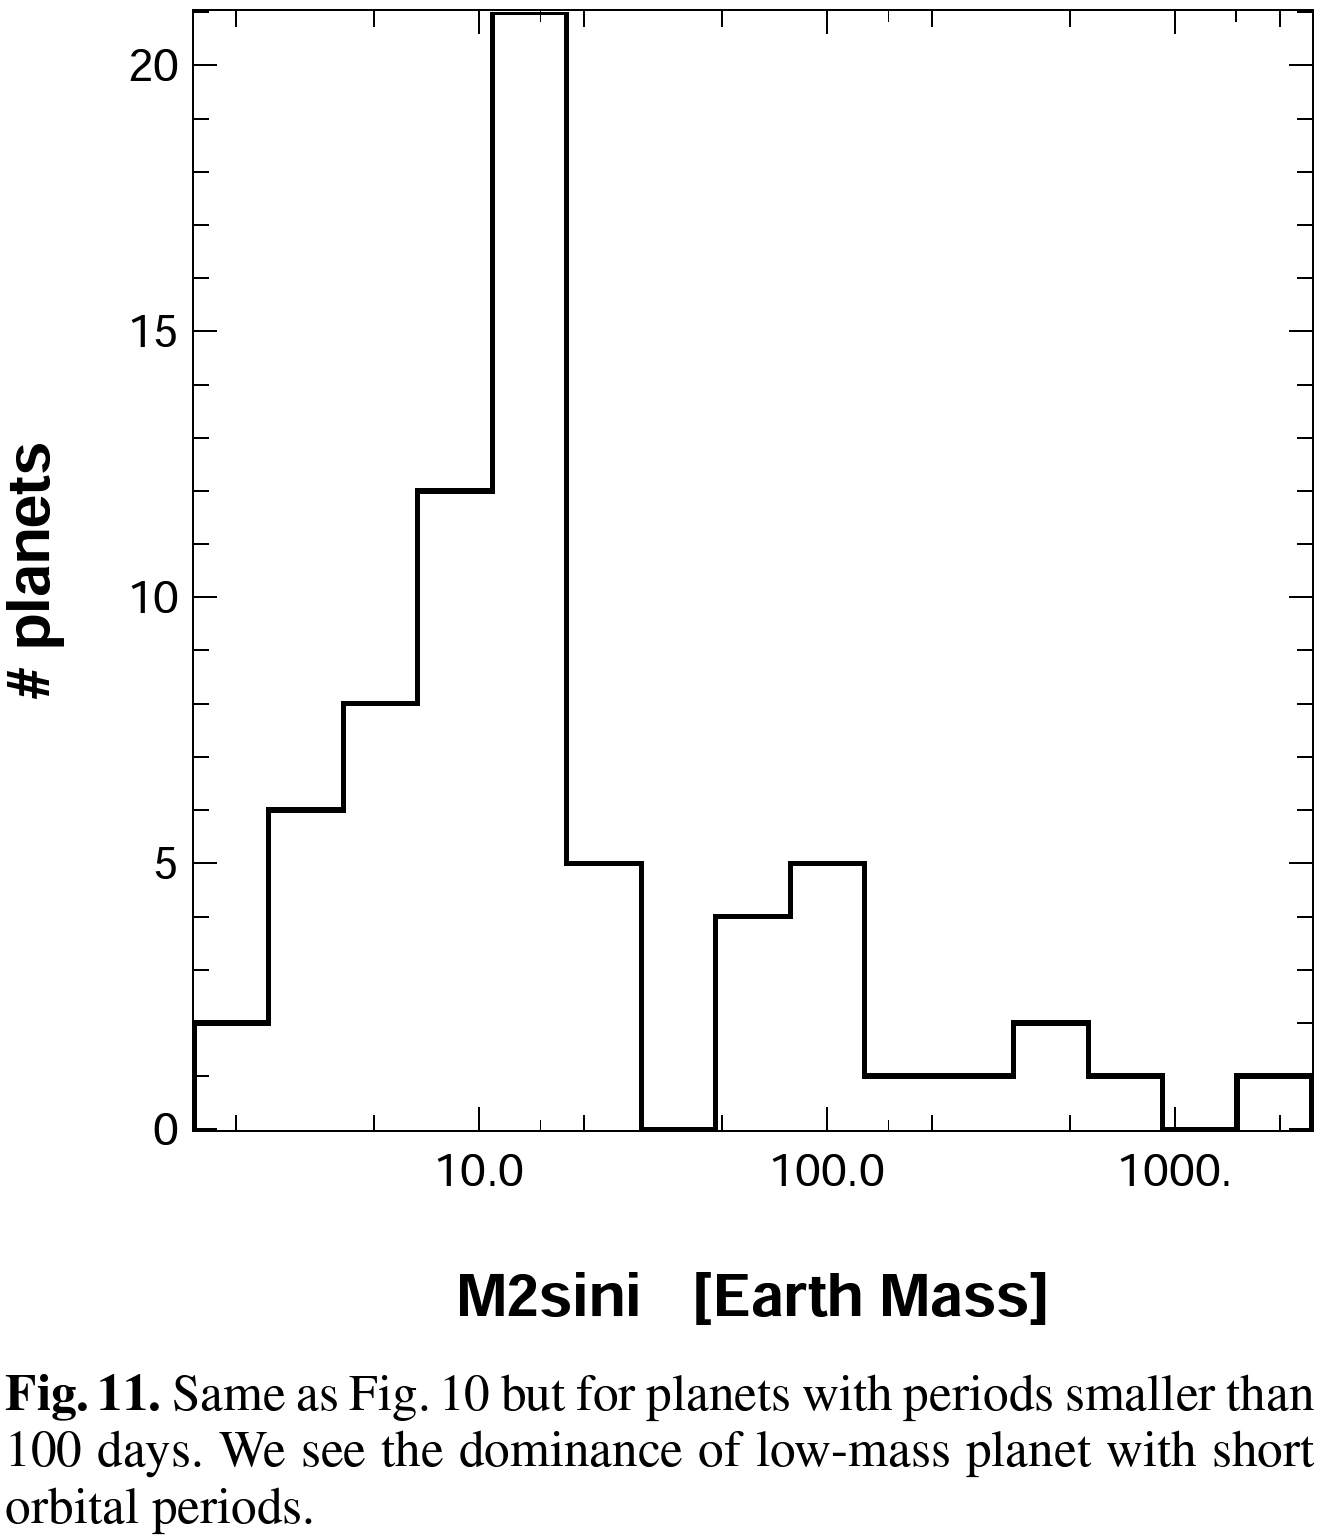
\includegraphics[trim={0cm 0 0 0},clip,height=0.45\textheight]{pvsMP100}\label{fig:pvsMP100}
\end{subfigure}
\end{figure} 

\begin{figure}[!ht]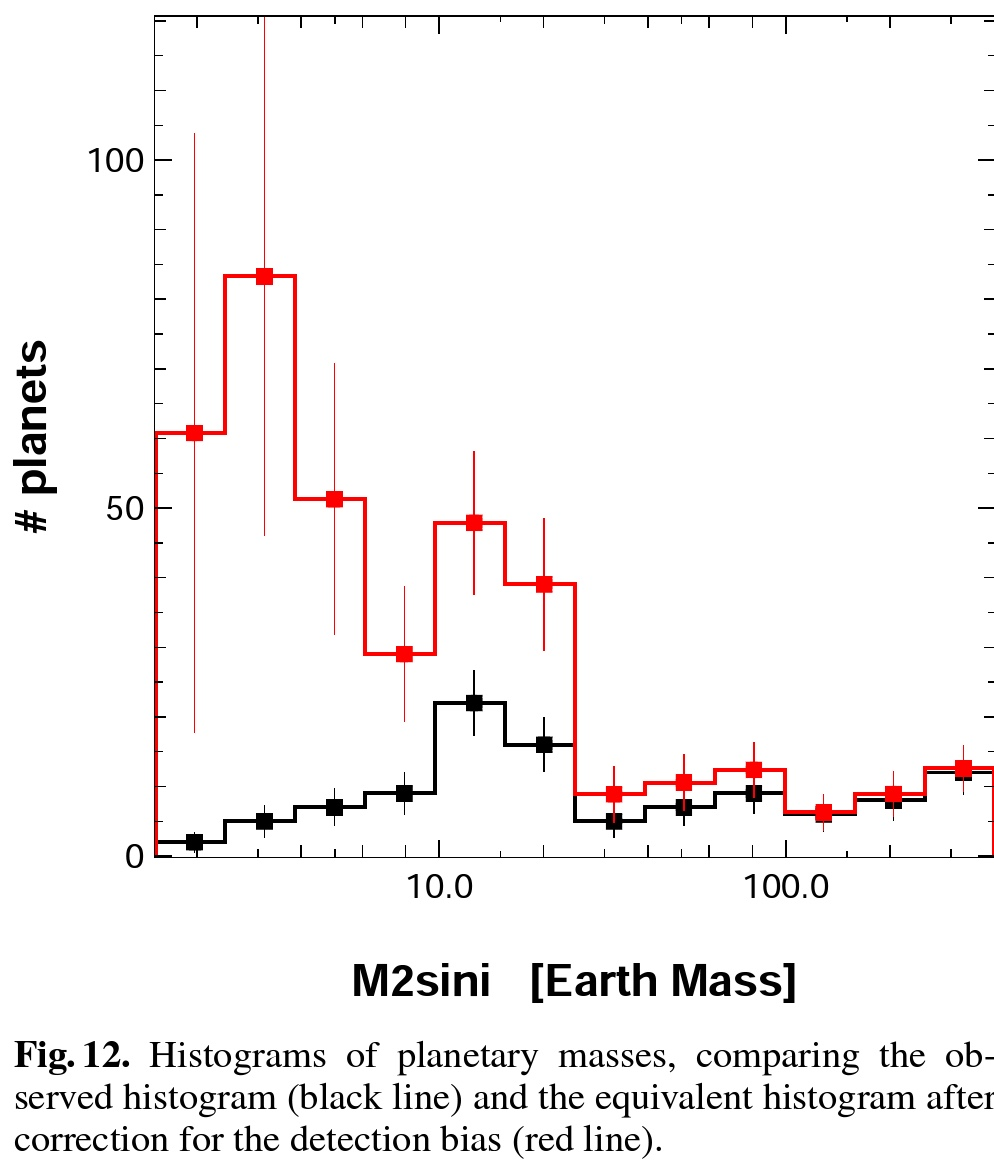
\includegraphics[trim={0cm 0cm 0 0},clip, keepaspectratio,height=0.45\textheight]{freqvsM}\label{fig:freqvsM}
\end{figure}

\end{frame}

\begin{wordonframe}{Distribuzione masse}
Gap nella distribuzione di massa attorno a $30\mearth{}$, popolazione di pianeti con massa minore di $10\mearth{}$ con $P<\SI{100}{\day}$, distribuzione piatta in $\log{M}$ nel range $30\mearth{}-4\mjupiter{}$.
\end{wordonframe}

\begin{frame}{Distribuzione periodi planetarii (a): RV, Mayor 11}
\begin{figure}[!ht]
\begin{subfigure}[b]{0.47\textwidth} \centering 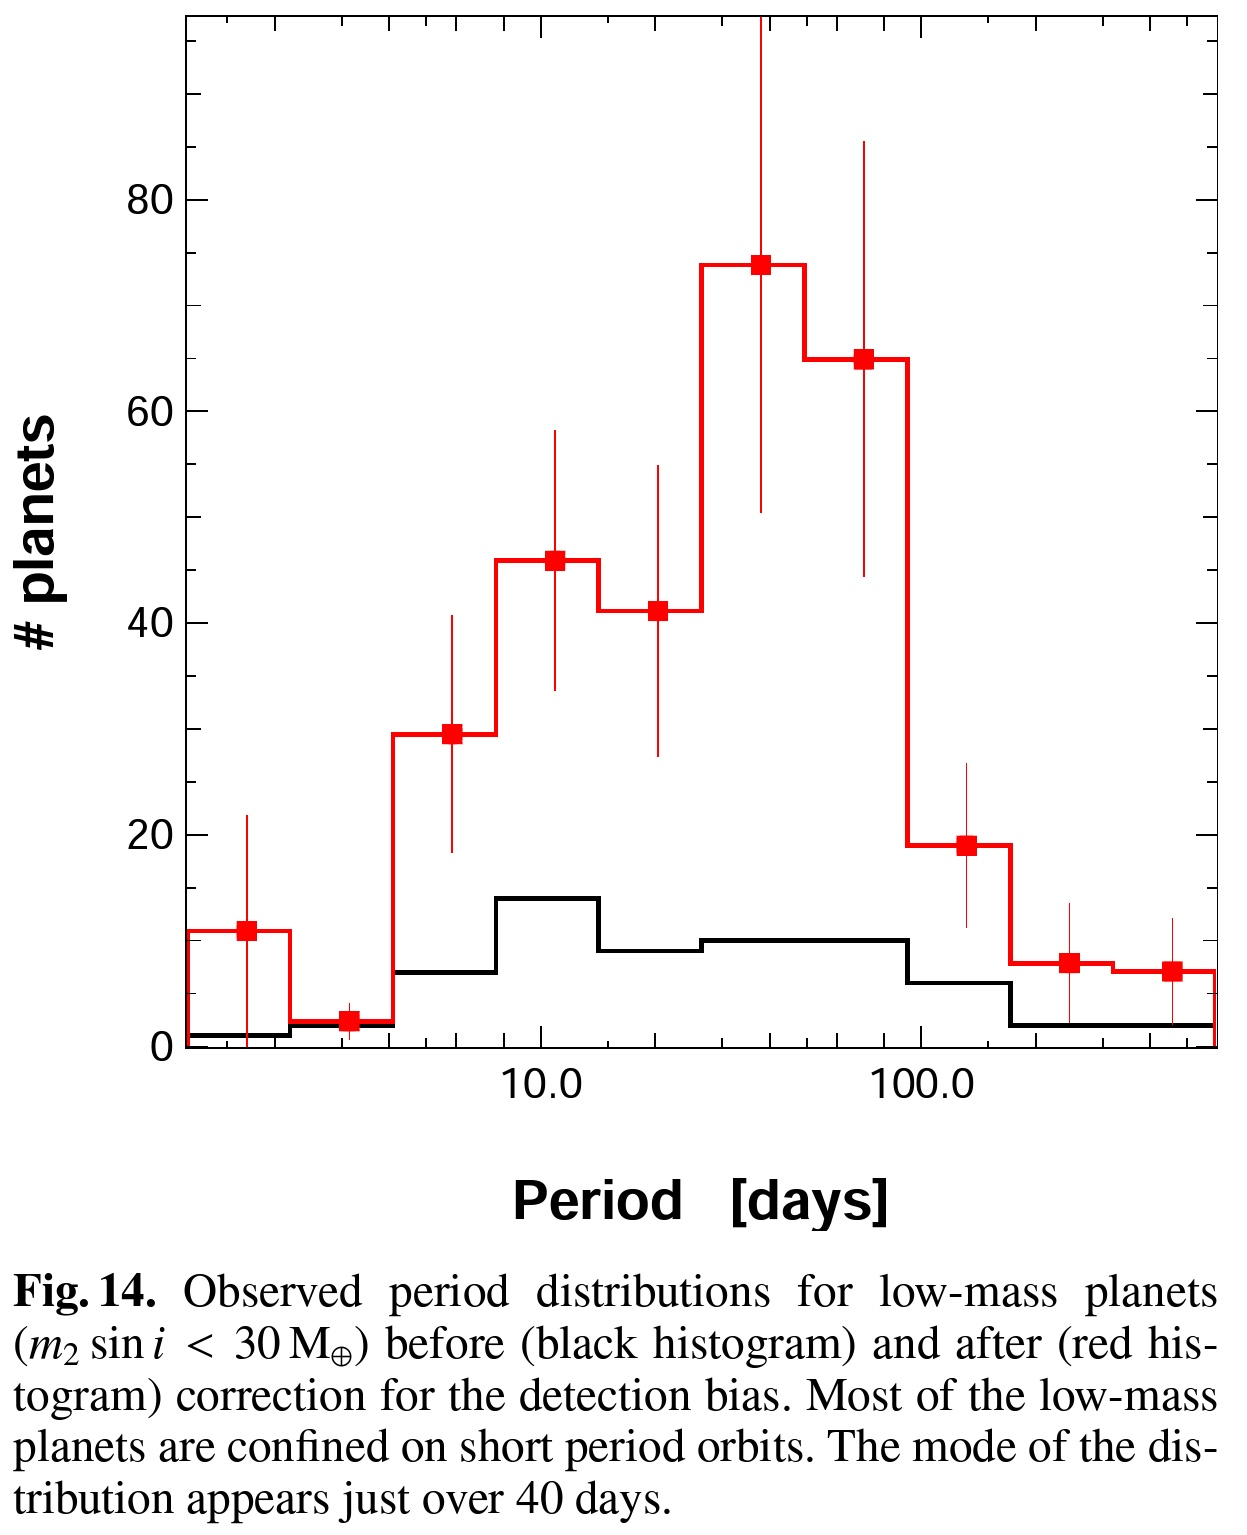
\includegraphics[trim={0cm 0 0 0},clip,width=0.99\textwidth]{freqvsPlowM}\label{fig:freqvsPlowM}\end{subfigure}
~
\begin{subfigure}[b]{0.47\textwidth} \centering 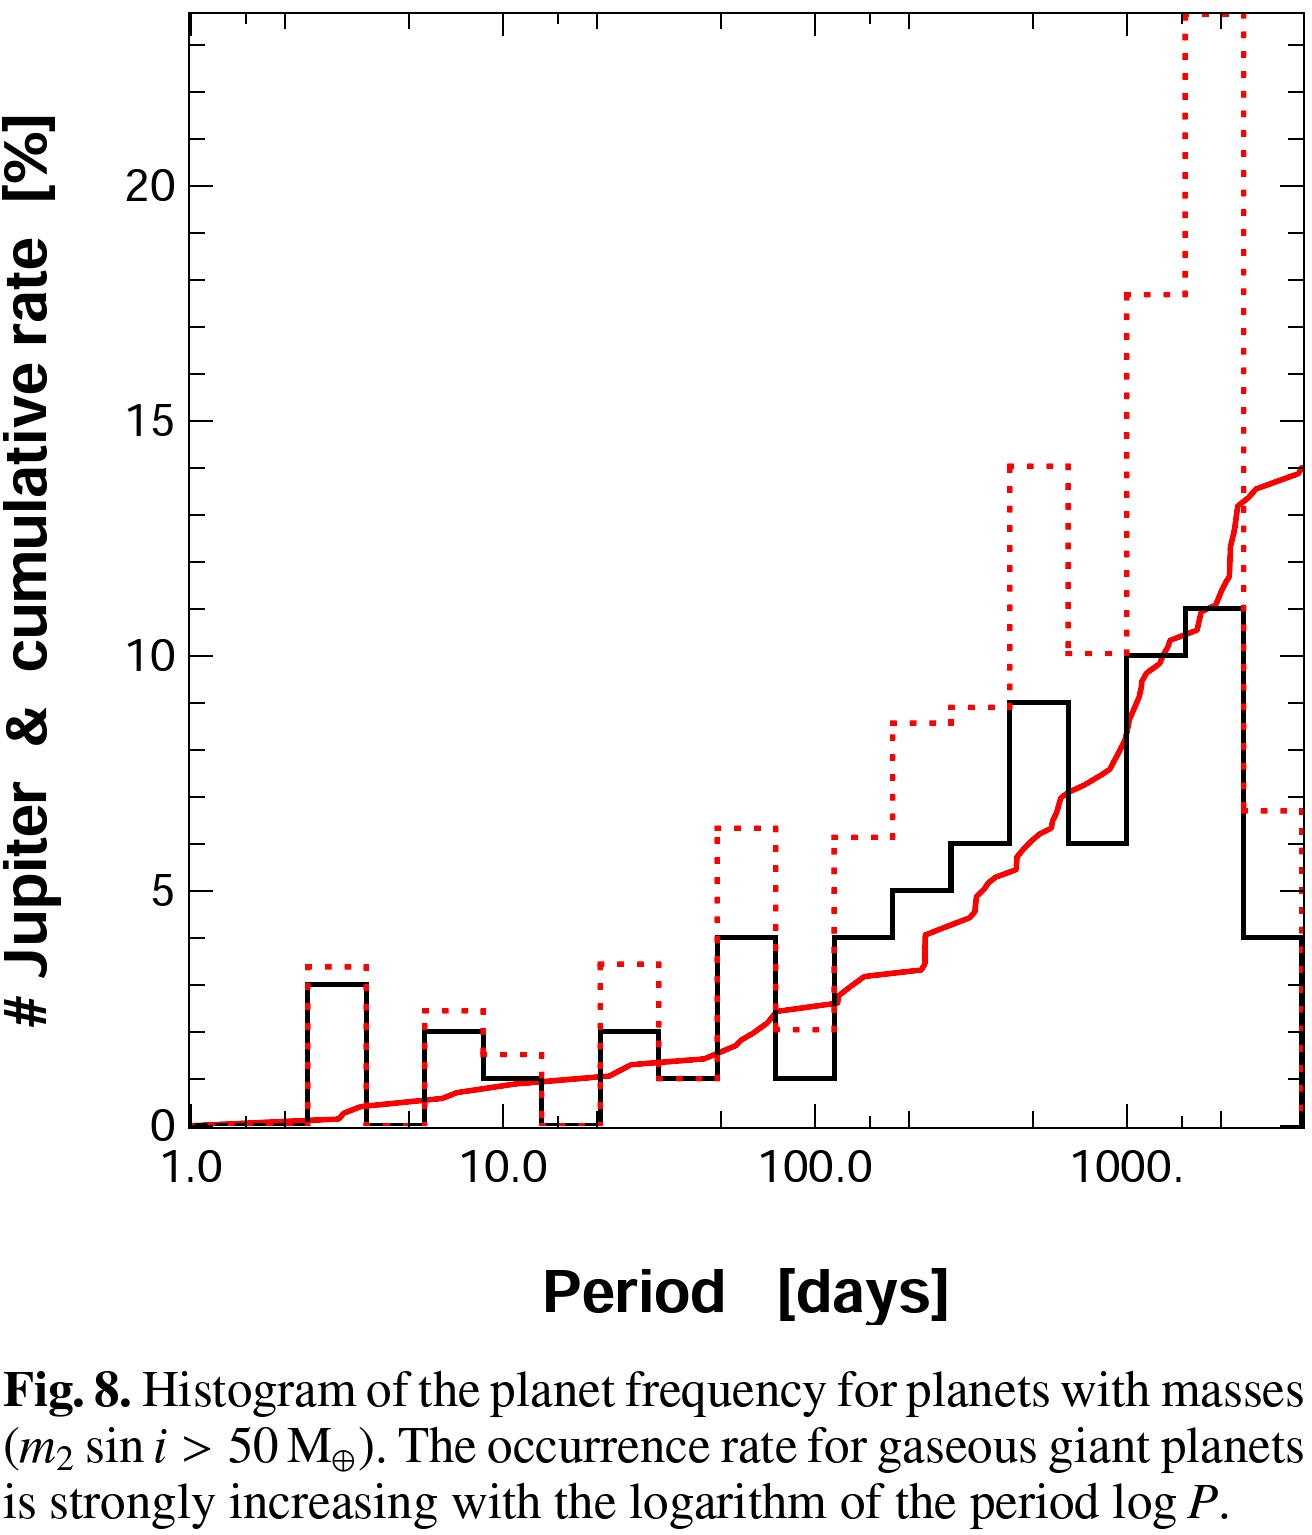
\includegraphics[trim={0cm 0 0 0},clip, height=0.5\textheight]{freqvsPgiant} \label{fig:freqvsPgiant} \end{subfigure}
\end{figure}
\end{frame}

\begin{wordonframe}{Distribuzione periodi}
I pianeti giganti sono raggruppati attorno a \SI{3}{\day}, possibile minimo entro \SI{100}{\day} e distribuzione che cresce rapidamente dopo \SI{100}{\day}.
Pianeti $M<30\mearth{}$ concentrati in \SIrange{10}{100}{\day}.
\end{wordonframe}

\begin{frame}{Caratteristiche orbitali: RV, Mayor 11}
\begin{figure}[!ht]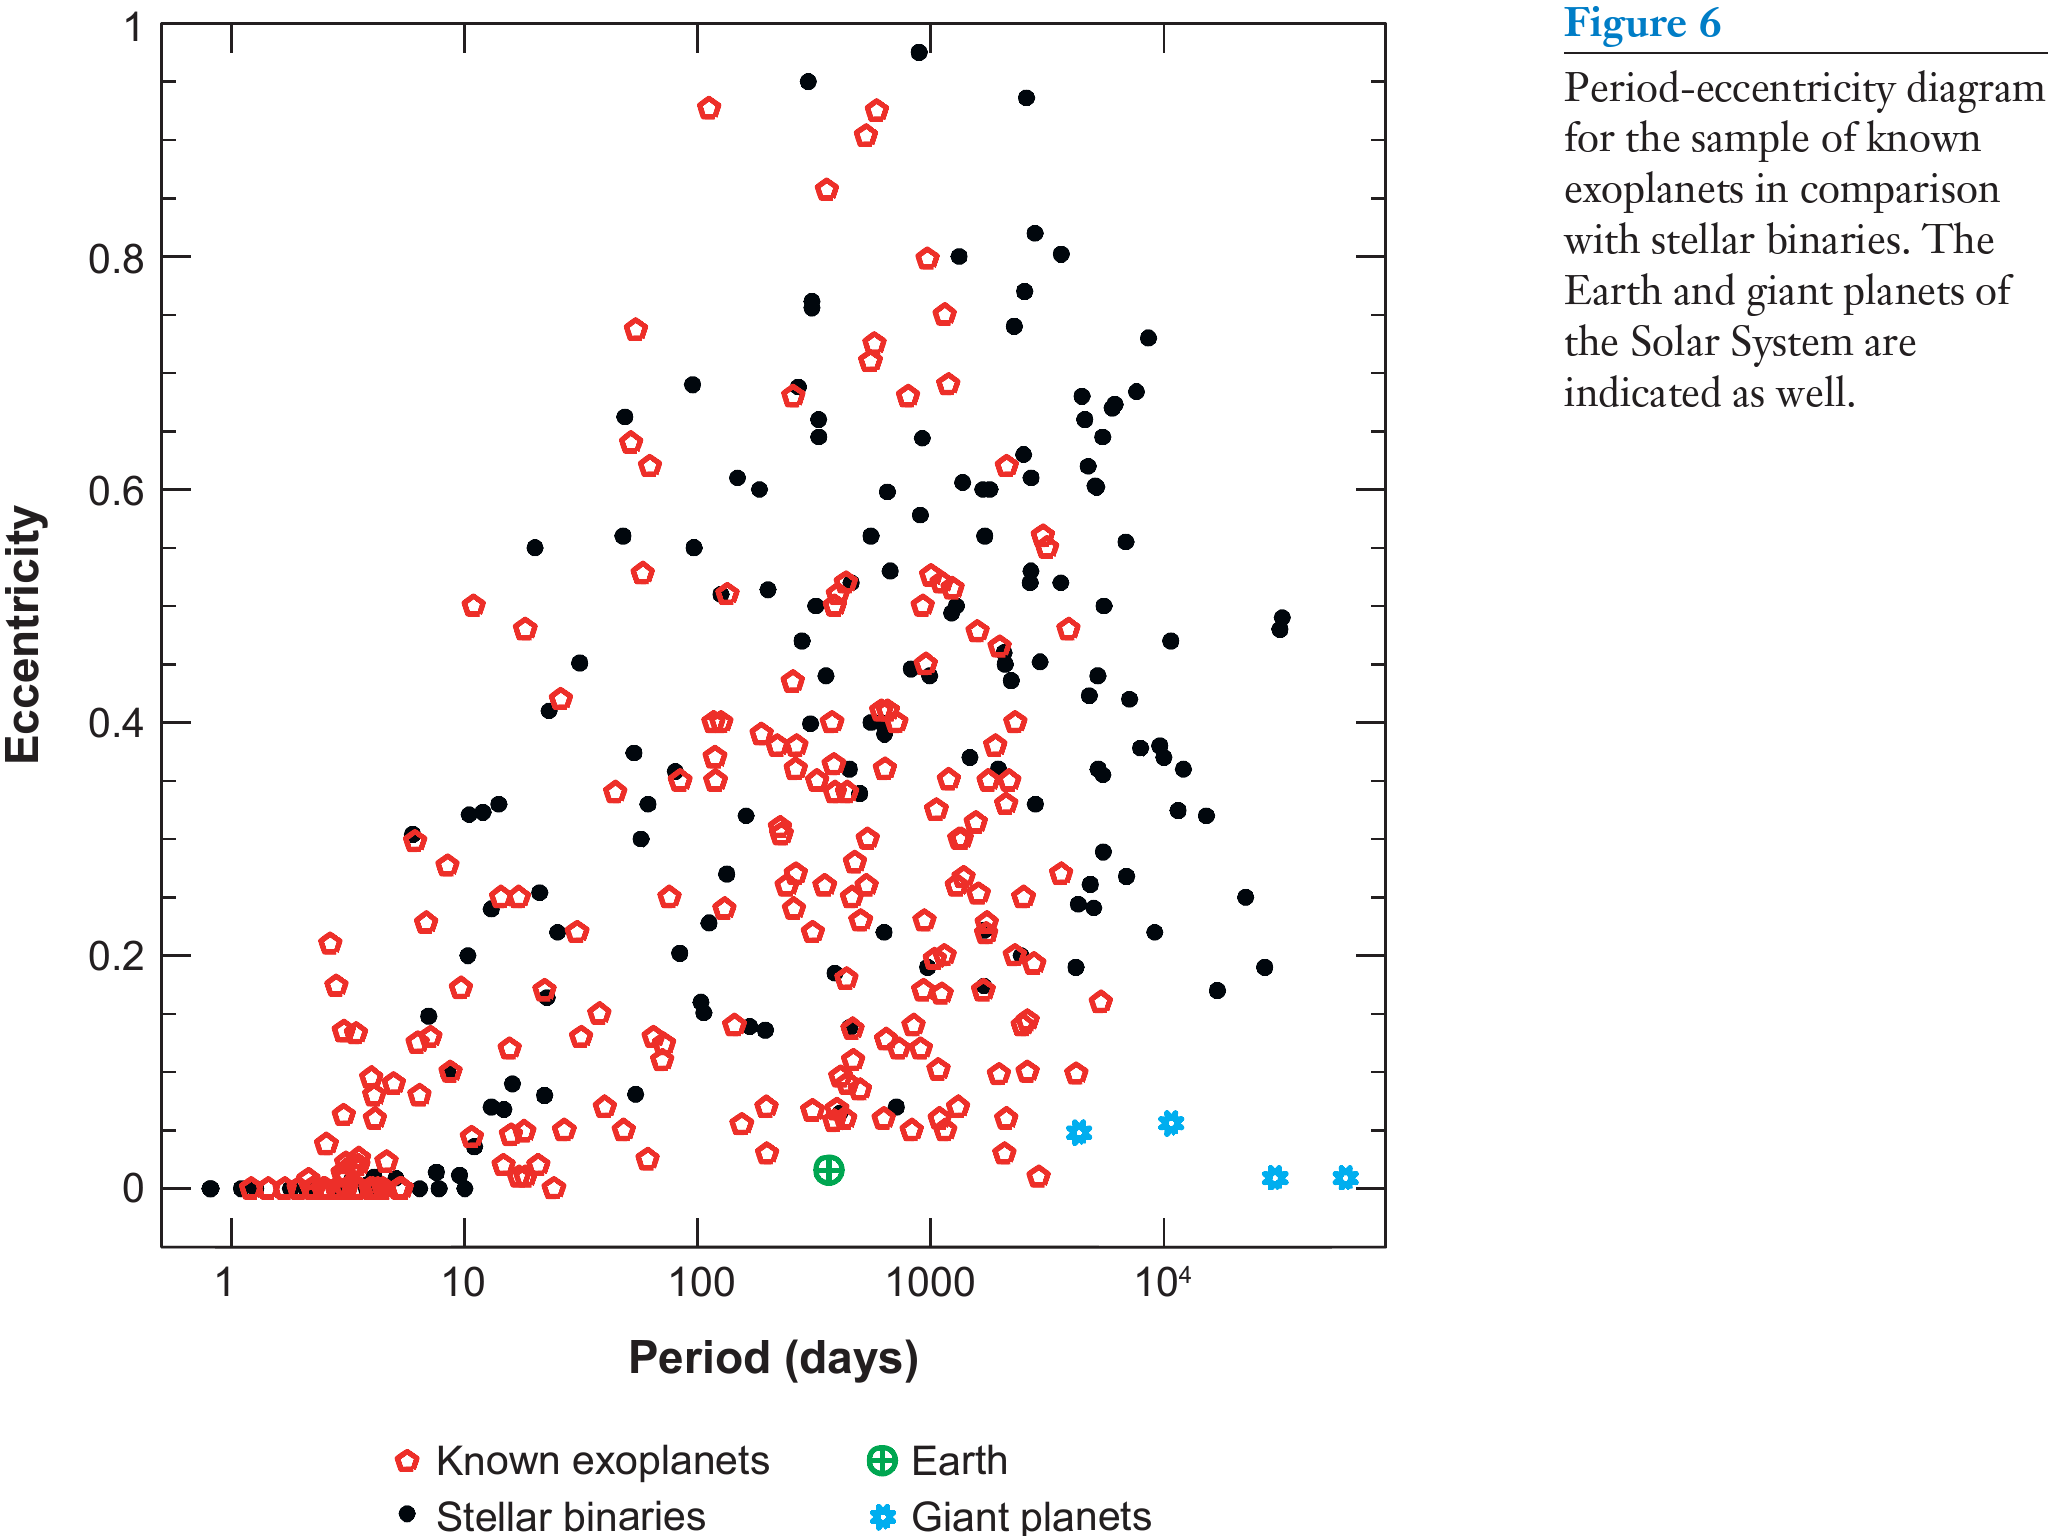
\includegraphics[trim={0cm 0cm 0 0},clip, keepaspectratio,width=0.5\textwidth]{eP}\label{fig:eP}\end{figure}
$\exv{e}\approx0.29$ - binary stars.

\begin{columns}[T]\begin{column}{0.5\textwidth}
Large scattering of e for gas giant (up to 0.93), up to $0.45$ for $M<30\mearth{}$.
\end{column} \begin{column}{0.5\textwidth}
\begin{equation*}
dN=S(x,\sigma_x)\,dx=\frac{x}{\sigma_x^2}\exp{-\frac{x^2}{2\sigma_x^2}} 
\end{equation*}
\end{column}  \end{columns}

\end{frame}

\begin{wordonframe}{Propriet\'a orbitali}
Fuori dalla regione di circolarizzazione mareali, $P=\SIrange{10}{30}{\day}$, ci sono comunque sistemi con piccola e (Sistema solare): evoluzione nel disco proto-planetario.
Sistemi con grande eccentricit\'a con $P=\SIrange{6}{10}{\day}$: influenza di compagno a grande periodo.
Planet-Planet scattering: upper part follow Rayleigh distribution.
\end{wordonframe}

\begin{frame}{Sistemi multipli e metallicit\'a}

\begin{figure}[!ht]
\begin{subfigure}[b]{0.47\textwidth} \centering 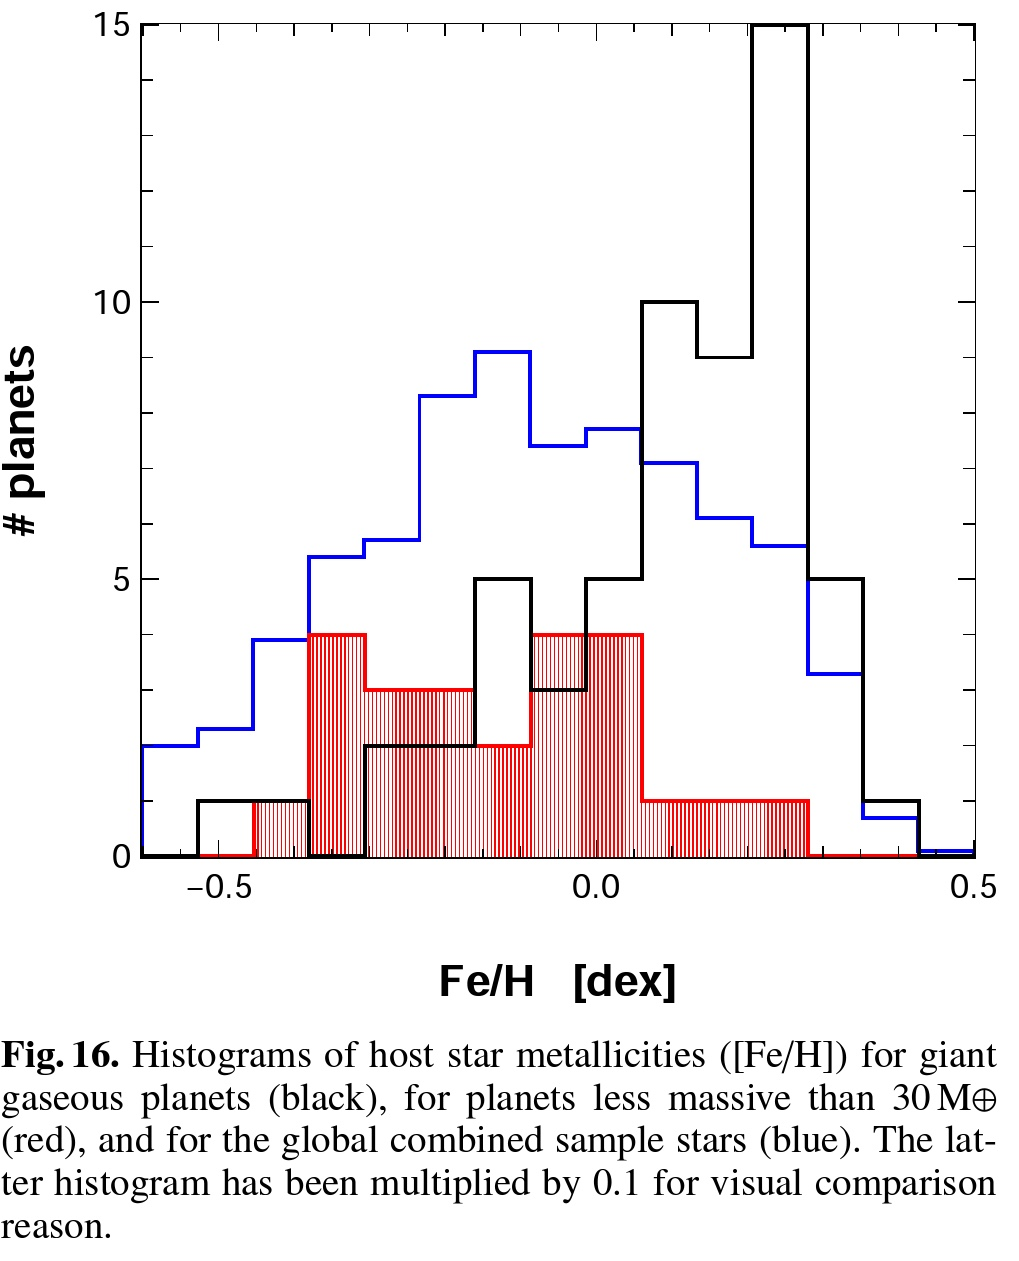
\includegraphics[trim={0cm 0 0 0},clip, height=0.45\textheight]{pvsFeH}\label{fig:pvsFeH} \end{subfigure}
~
\begin{subfigure}[b]{0.47\textwidth} \centering 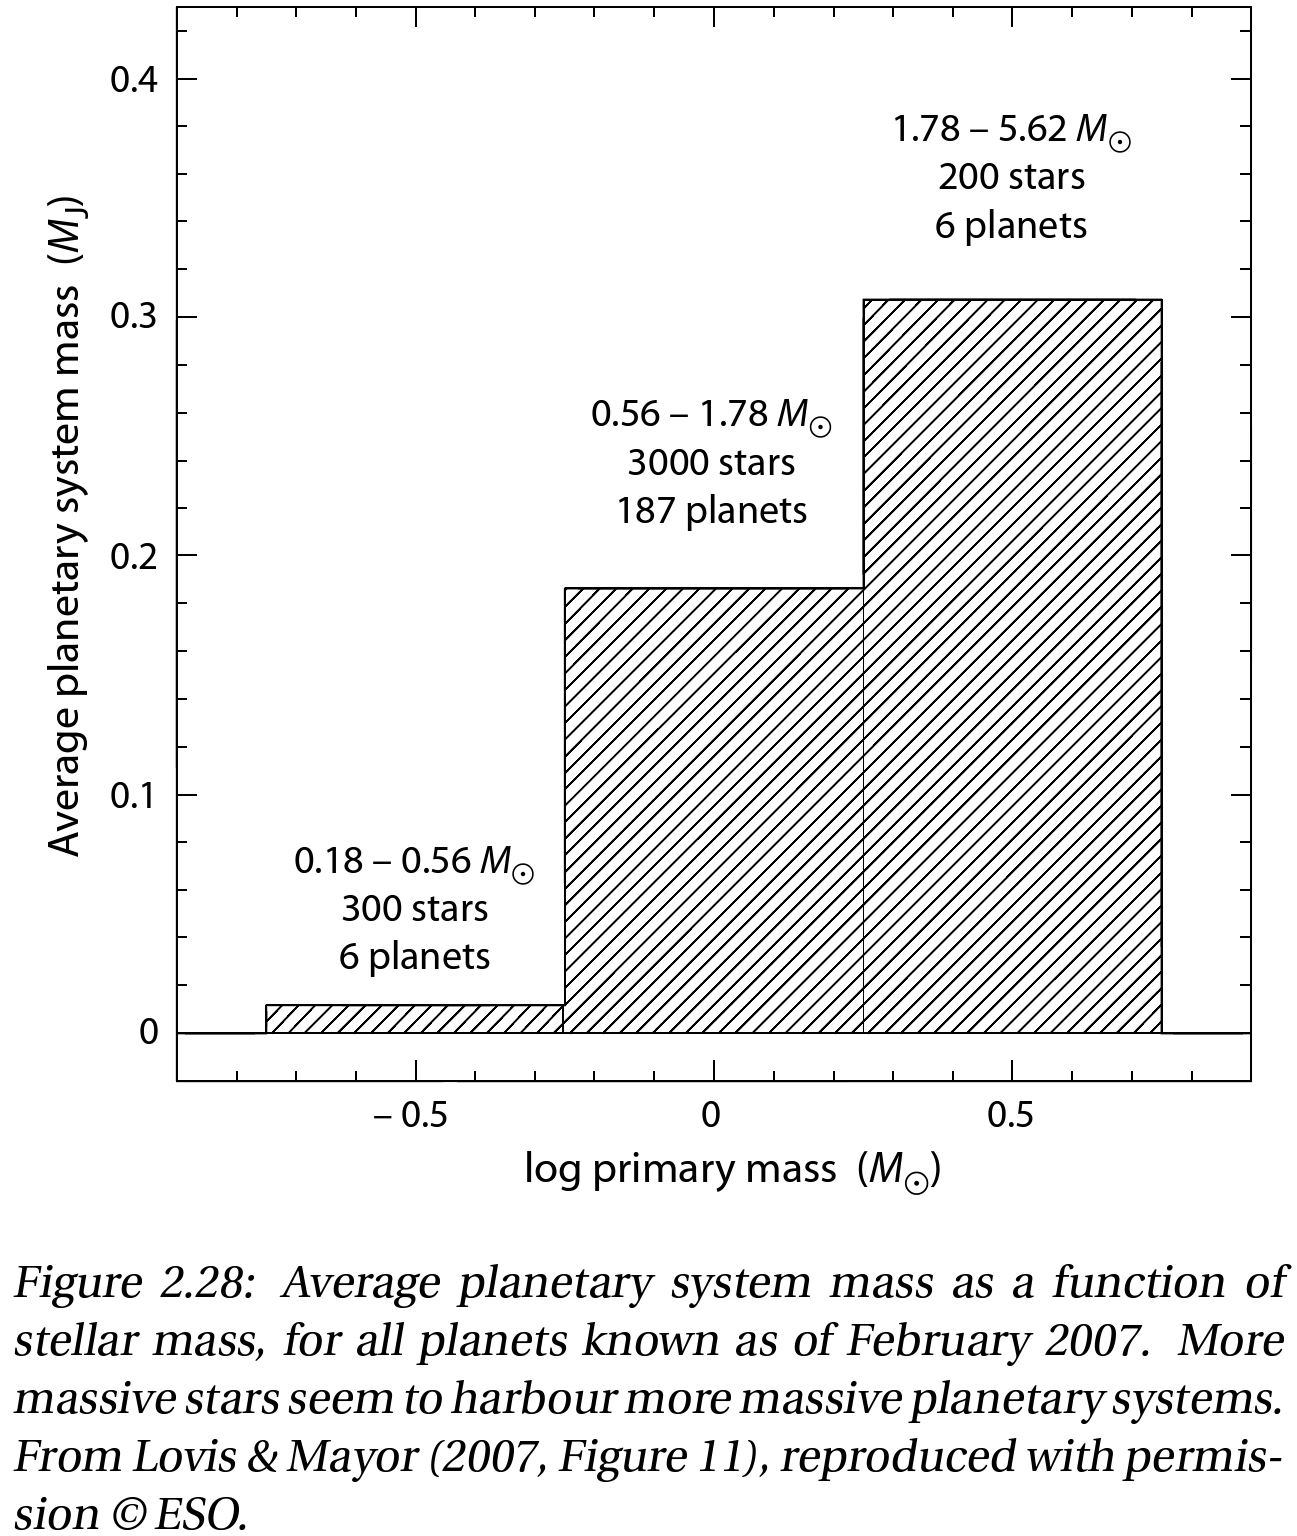
\includegraphics[trim={0cm 0 0 0},clip,height=0.45\textheight]{pMstar}\label{fig:pMstar}\end{subfigure}
\end{figure}
\begin{figure}[!ht]
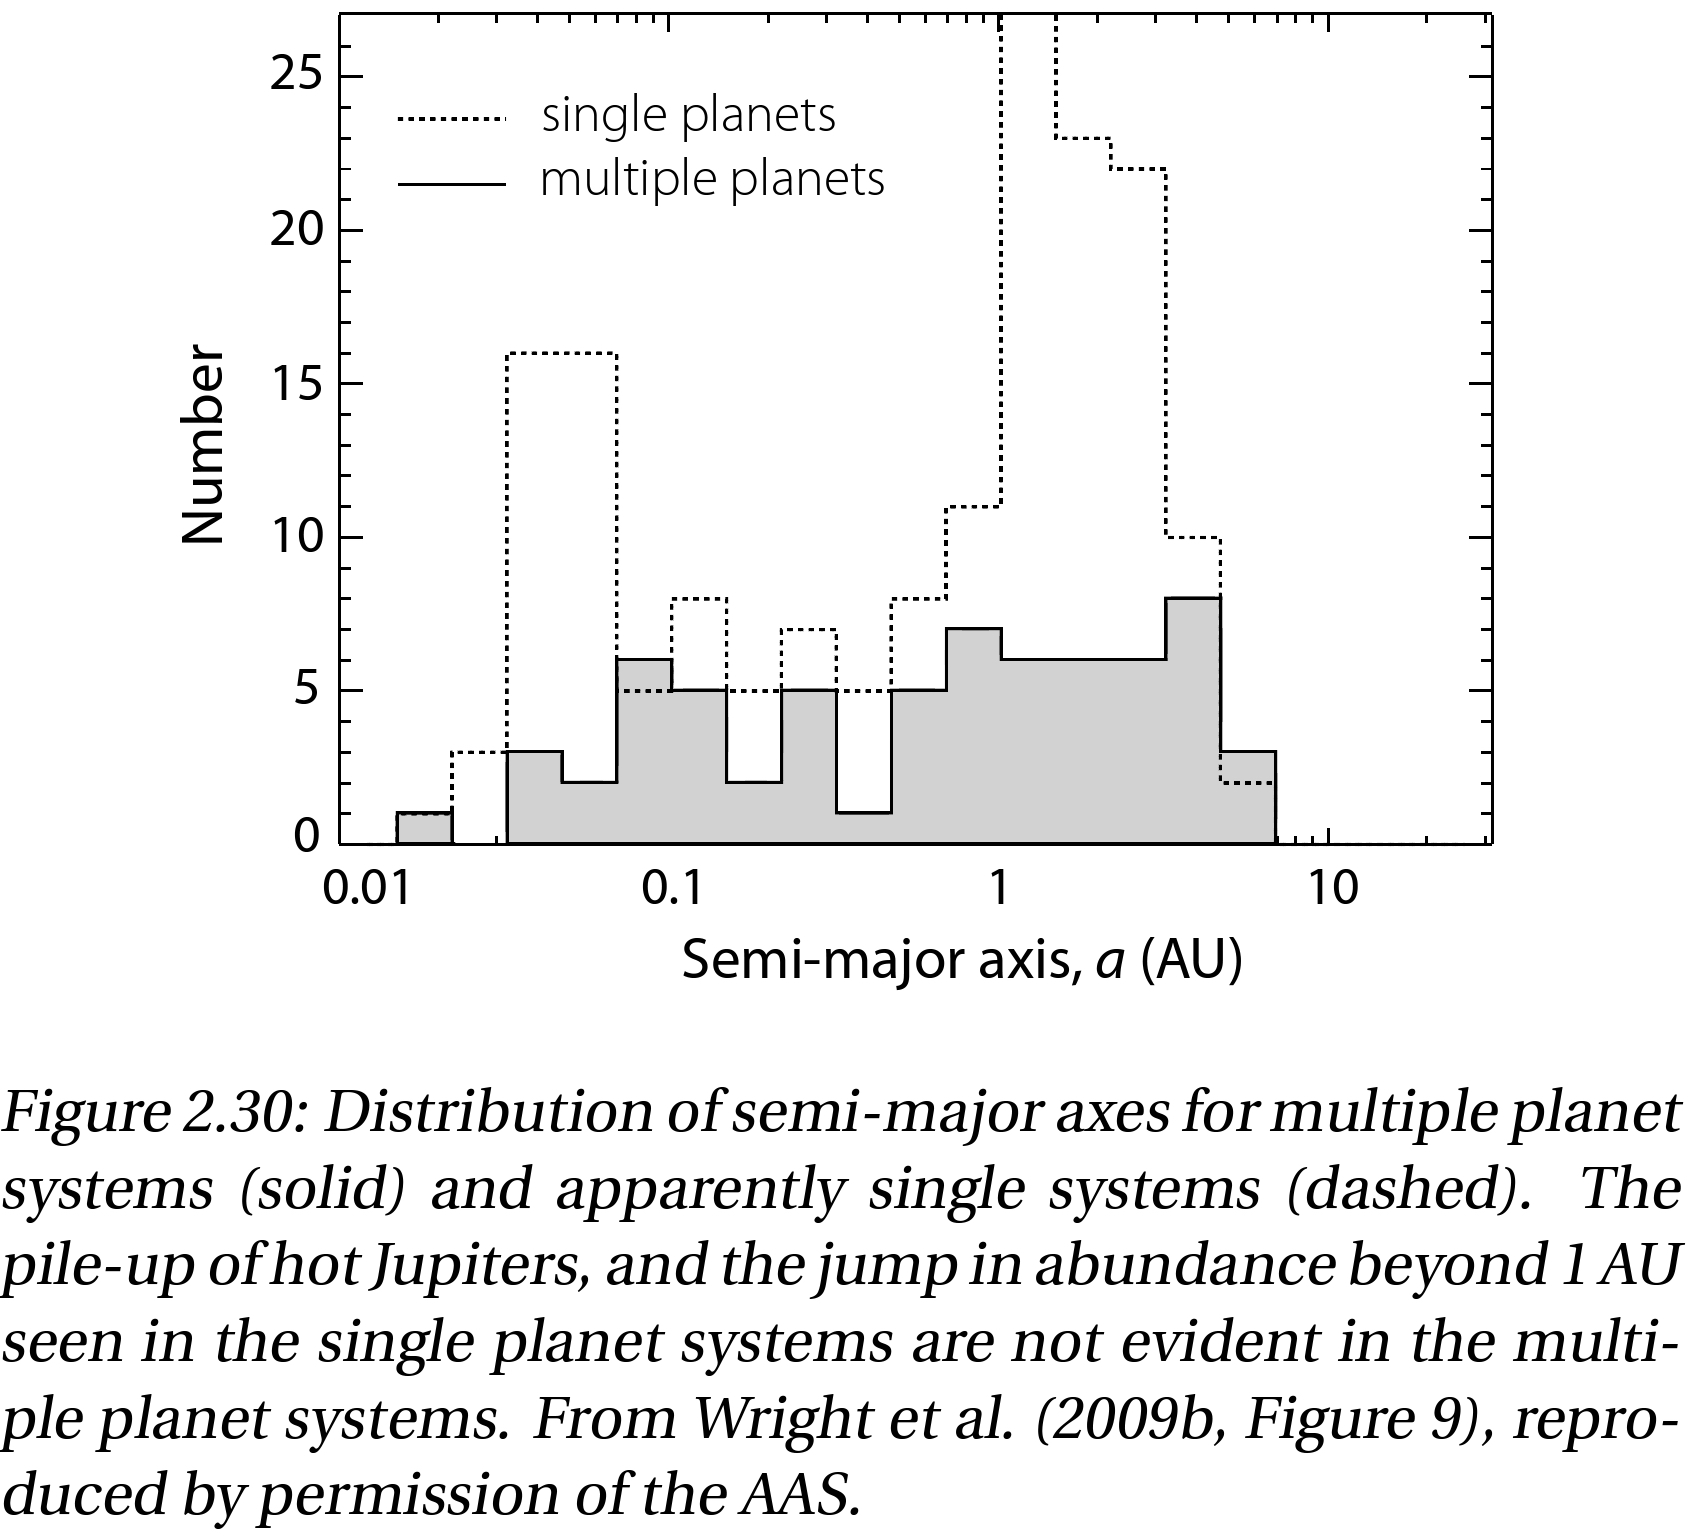
\includegraphics[trim={0cm 0cm 0 0},clip, keepaspectratio,height=0.45\textheight]{a-single-multi}\label{fig:a-single-multi}\end{figure}
\end{frame}

\begin{wordonframe}{Correlazione con caratteristiche stellari e sistemi multipli}
La frequenza dei pianeti giganti aumenta con la metallicit\'a stellare (Santos 04, Fischer Valenti 05); inoltre cresce nel range $1-2\msun{}$.
I sistemi multipli possono essere classificati in maniera non esclusiva secondo il numero di pianeti giganti, la presenza di MMR, secondo l'importanza delle interazioni pianeta-pianeta, la presenza di pianeti sub-gioviani.
La distribuzione dei periodi nei sistemi multipli mostra accumulo meno pronunciato a \SI{3}{\day}, e \SI{1}{\astronomicalunit}
\end{wordonframe}


\section{Properties of transit exoplanets}

\begin{frame}{Distribuzione raggio planetario}
\begin{columns}  \begin{column}{0.5\textwidth}
\begin{figure} \centering 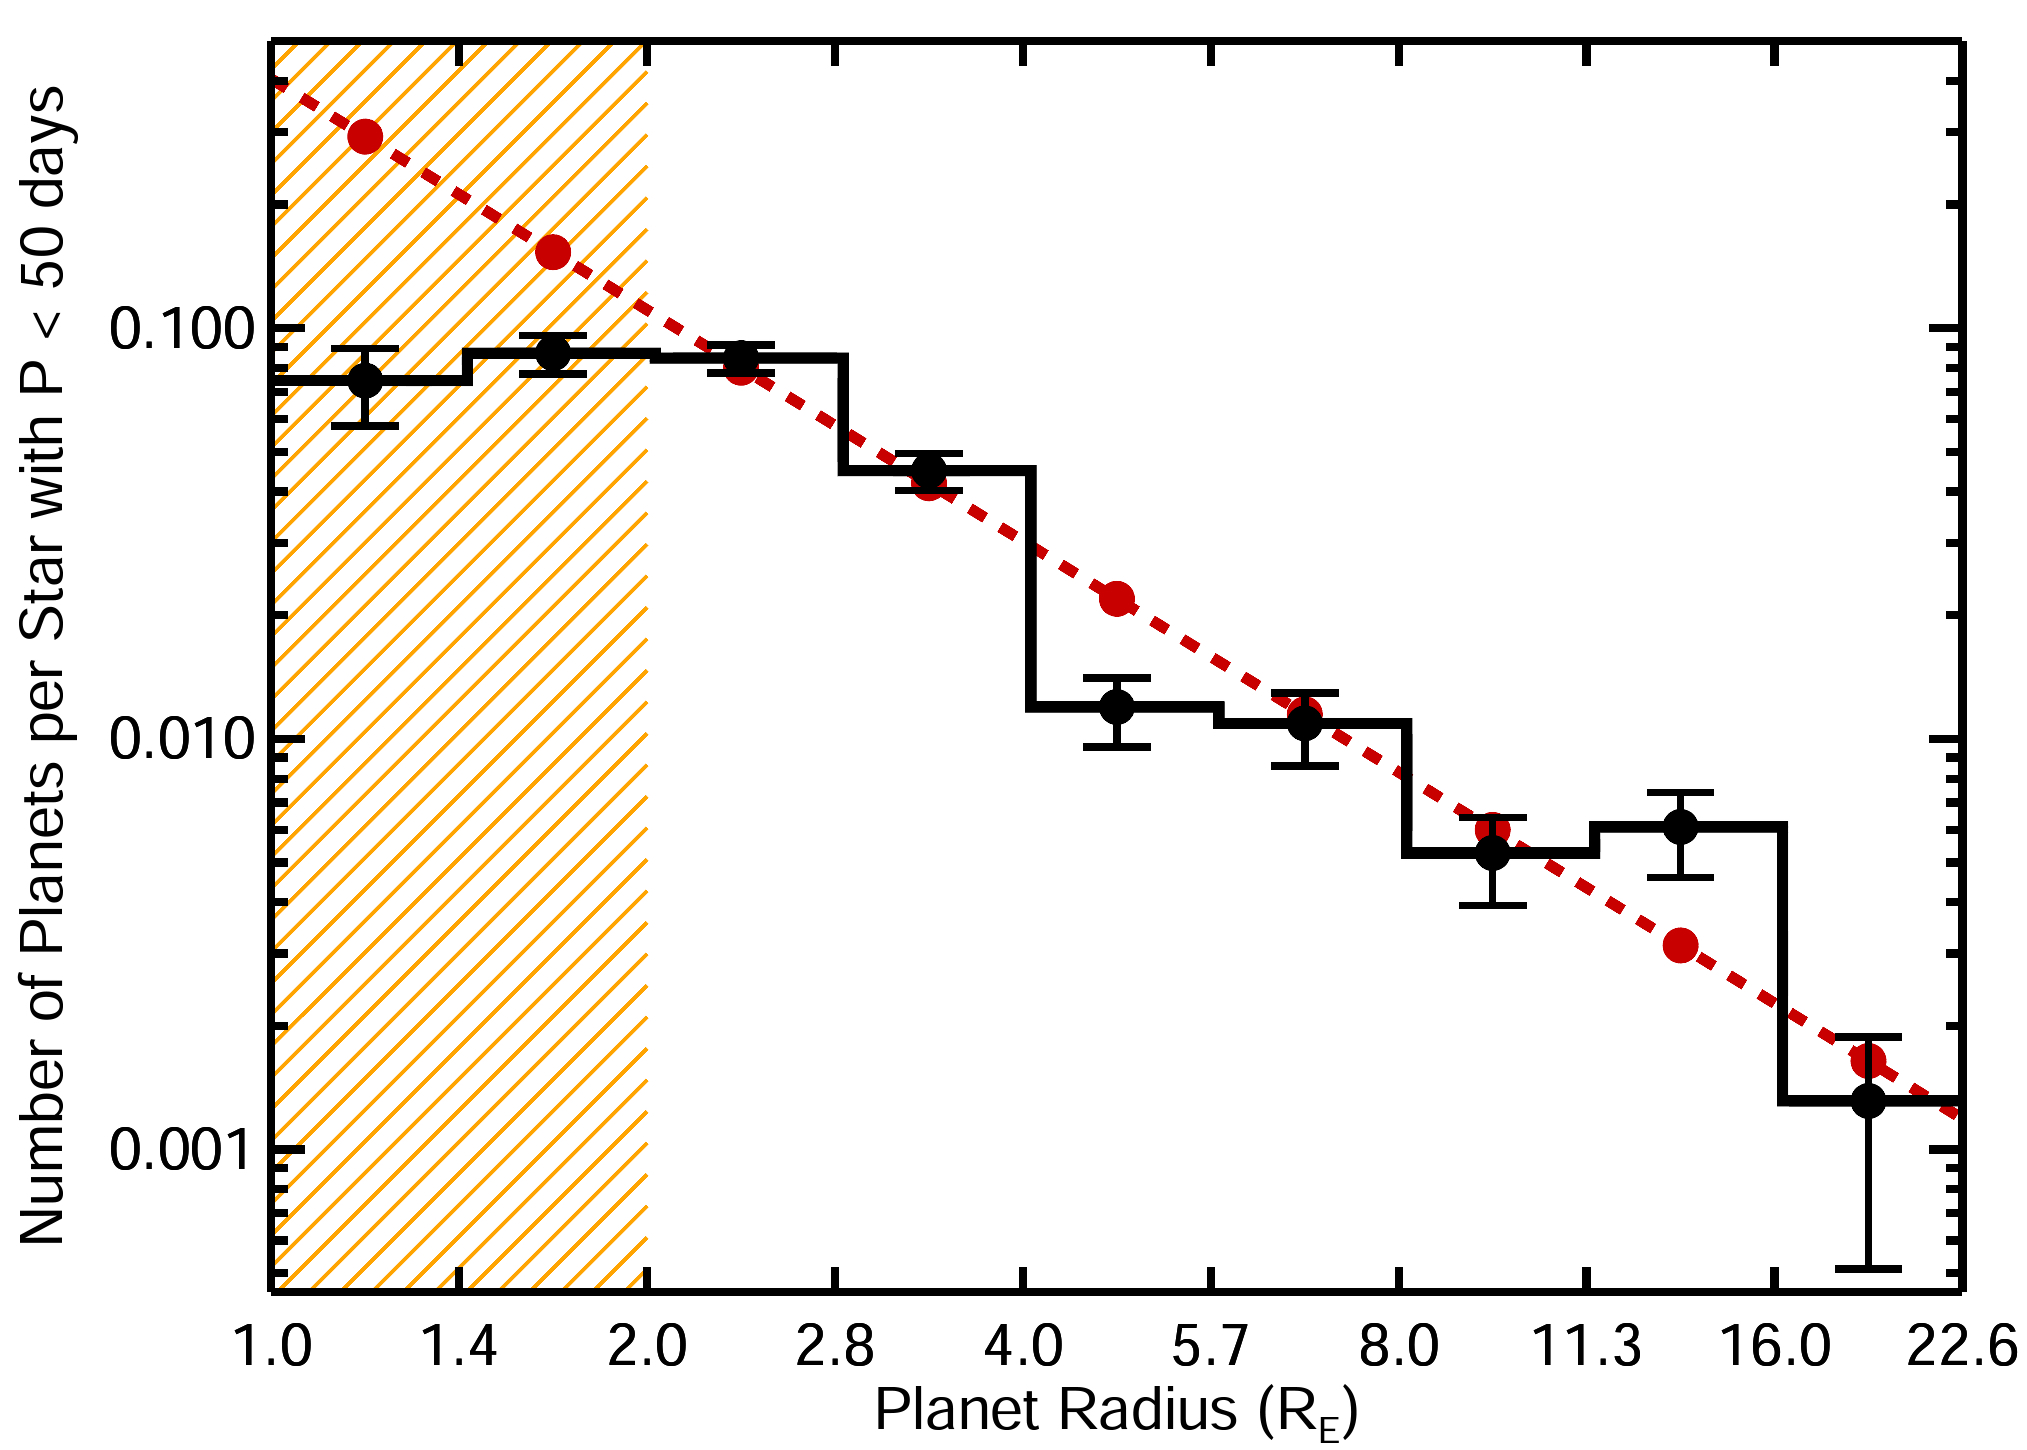
\includegraphics[trim={0cm 0 0 0},clip, height=0.45\textheight]{freqvsRpl50l} \label{fig:freqvsRpl50l}
\end{figure}

\begin{figure}
\centering \includegraphics[trim={0cm 0 0 0},clip,height=0.45\textheight]{freqvsRpl50}\label{fig:freqvsRpl50}\end{figure} 
\end{column} \begin{column}{0.5\textwidth}
\cite{howard2012planet}: $P<\SI{50}{\day}$, $R=\range{2}{22.7}\rearth{}$
\begin{equation*}

\end{equation*}
\end{column}  \end{columns}
\end{frame}

\section{Orbital evolution}

\subsection{Hot Jupiters due to tidal circularization}

\begin{frame}{Planet-Planet scattering}
Scattering in eccentric close-in orbit. Tidal circularization: limit distance twice the Roche limit.
\end{frame}

\begin{wordonframe}{Tidal circularization}
During circularization angular momentum $\propto \sqrt{GMa(1-e^2)}$: for $e\approx1$: $a_f=a_i(1-e^2)\approx2a_{peri}$.

$R_p=0.462a_R(\frac{M_p}{M_*})\expy{\frac{1}{3}}$ 
\end{wordonframe}



%%%Appunti penco
\part{Dinamica/Meccanica celeste}

\chapter{Problema a 2 corpi}
\PartialToc

\section{Problema dei 2 corpi}

\subfile{tikz/reducedproblem.tex}

\begin{usefull}{Costante di Gravitazione universale: G}

\begin{equation*}
G\approx4.302*10^{-3}\,pc/M_{\odot}^{3}(km/s)^2
\end{equation*}

\end{usefull}

\subsection{Problema ridotto}


\subsubsection{Legge di gravitazione}

La forza che agisce sui 2 corpi \'e risp
\begin{align*}
\vec{F_m}=-GMm\frac{\vec{r}}{r^3}\\
\vec{F_M}=-GMm\frac{\vec{r}}{r^3}\\
\end{align*}

\begin{definition}{Coefficiente $\gamma$ del problema a 2 corpi}

Definisco $\gamma=GmM$. G \'e la costante di gravitazione universale.

\end{definition}


Ridurremo il problema a 2 corpi al problema di un corpo di massa $\mu$ attratto da un centro $O$
\begin{align*}
m\ddvec{r_1}=\vec{F_m}=-GMm\frac{\vec{r}}{r^3}\\
M\ddvec{r_2}=\vec{F_M}=-GMm\frac{\vec{r}}{r^3}\\
\end{align*}
dividendo e sottraendo si perviene all'equazione fondamentale

\begin{align}
&\mu\ddvec{r}=-\gamma\frac{\vec{r}}{r^3}\label{eq:fondamentale}\\
&\ddvec{r}=-k^2\frac{\vec{r}}{r^3}
\end{align}

Introduco la costante di Gauss\index{Costante di Gauss}
\begin{align*}
\frac{1}{\mu}=\frac{1}{M}+\frac{1}{M}\\
k^2=\frac{\gamma}{\mu}=G(M+m)
\end{align*}

\subsection{Costanti del moto: energia, momento angolare, vettore di Lenz}
Avendo come obiettivo di integrare ~\ref{eq:fondamentale} elenco le costanti del moto (Per primi due vedi moto a 2 corpi riferito al CM)

\begin{enumerate*}

\item Energia\\
\begin{equation*}
E=T+V=\frac{1}{2}\mu|\dot{r}|^2-\frac{\gamma}{r}
\end{equation*}

\item Momento angolare\\
\begin{equation*}
\vec{J}=\mu\vecp{r}{\dot{r}}
\end{equation*}
quindi \lbt{\scap{J}{r}=0}{\scap{J}{\dot{r}}=0} cio\'e il momento angolare \'e perpendicolare al vettore posizione e alla velocit\'a.


\item Vettore di Lenz\\
\begin{equation*}\label{eq:lenzv}
\vec{L}=\vecp{\dot{r}}{J}-\gamma\frac{\vec{r}}{r}
\end{equation*}


\subfile{tikz/lenzvector.tex}

\end{enumerate*}

Esplicitando $\vec{\dot{L}}$ e usando la conservazione dell'energia e l'equazione del moto ~\ref{eq:fondamentale} vedo che $\vec{L}$ \'e costante del moto.

\subsection{Propriet\'a del vettore di Lenz}

\begin{itemize*}
\item Ortogonale al mometno angolare
\begin{equation*}\label{eq:JLzero}
\scap{J}{L}=0
\end{equation*}

\item Modulo del vettore di Lenz
\begin{equation*}\label{eq:moduloL}
L^2=\gamma^2+\frac{2}{\mu}EJ^2
\end{equation*}

\item Proiezione di $\vec{L}$ lungo $\vec{r}$
\begin{equation*}\label{eq:Lr}
\scap{L}{r}+\gamma r=\frac{1}{\mu}J^2
\end{equation*}
\end{itemize*}

\subsection{Conseguenze delle leggi di conservazione}

\begin{enumerate*}
\item Moto piano\\
Esiste un vettore $\vec{J}$, costante del moto, sempre ortogonale ad $\vec{r}$: $\vec{r}$ ruota in un piano ortogonale a $\vec{J}$.
\item Il vettore di Lenz \'e sul piano dell'orbita\\
Segue da ~\ref{eq:JLzero}
\end{enumerate*}


\section{Forma dell'orbita}


\subsubsection{Anomalia vera}

Chiamo anomalia vera l'angolo tra $\vec{L}$ e $\vec{r}$.

Utilizzo ~\ref{eq:Lr} per ricavare l'equazione dell'orbita $r=\frac{\frac{J^2}{\mu}}{\gamma+L\cos{v}}$ e ponendo \lbt{p=\frac{J^2}{\gamma\mu}}{e=\frac{L}{\gamma}} ottengo la conica
\begin{equation*}\label{eq:orbitaconica}
r=\frac{p}{1+e\cos{v}}
\end{equation*}

\begin{itemize*}
\item $e>1$: Iperbole.

Deve essere $L>0\Rightarrow E=T+V>0$ e poich\'e \lbt{V<0}{V\abc{r\to\infty}{0}} il corpo pu\'o arrivare all'infinito con una certa energia cinetica

\item $e=1$: parabola.

Il corpo pu\'o andare all'infinito con velocit\'a tendente a zero.

\item $e<1$: ellisse.

Deve essere $L<\gamma\Rightarrow E<0$ (segue da ~\ref{eq:moduloL}): il corpo non pu\'o andare all'infinito dato che si avrebbe $T<0$.

\end{itemize*}

\subsection{Significato fisico del vettore di Lenz}

L'asse della conica \'e lungo $\vec{L}$; il modulo non ci da altre informazioni dato che dipende da $E$ e da $|\vec{J}|$ 



\section{Leggi di Keplero}



\section{Soluzione del moto}
Cenno i sistemi di coordinate Equatoriali ed Eclittiche - Soluzione del moto: anomalia vera, eccentrica, media - Approssimazioni per piccole eccentricit\'a - 

\section{ degli elem. orbitali da tre osservazioni (metodo di Laplace) }
Elementi dell'orbita di un pianeta (Tabella del sistema solare) - Determinazione degli elem. orbitali da tre osservazioni (metodo di Laplace) 

\section{effemeridi}
Riepilogo del problema dei due corpi - Calcolo delle effemeridi


\section{Stelle doppie.}
\begin{todo}{roche surface}
stellar interior: pg 107-109
\end{todo}


\chapter{Problema dei 3 corpi}


Problema ristretto dei tre corpi: Riferimento rotante, Integrale di Jacobi, superfici di Hill - Punti di Lagrange 
\PartialToc

\section{Riferimento rotante}

Determinazione e stabilit\'a dei punti Punti di Langrange - Cenno alla stabilit\'a delle config. gerarchiche - Asteroidi Troiani e Greci - Problema delle comete - Criterio di Tisserand - Elementi e valori numerici del sistema Sole-Terra-Luna.
Campo delle forze di marea - Sistema Terra-Luna-Sole - Cenno alle maree terrestri
Perturbazione da primario non sferico: campo di forze aggiuntivo - Effetto sul periodo, sul nodo ascendente, sulla posizione del perigeo. - Precessione lunisolare - 


\stopcontents[chapters]


\backmatter

\part{Appendice}

\chapter{Programma Astrofisica/a 2016}

\begin{itemize}
    \item equilibrio idrostatico: sistemi autogravitanti.
    
Sistemi autogravitanti; l'equazione dell'equilibrio idrostatico. La scala di tempo dei processi dinamici: il tempo di free fall.

\item Modelli politropici e applicazioni: l'equazione di eddington e il peso della pressione di radiazione sull'equilibrio di una stella. 

Modelli politropici di nane bianche e stelle di neutroni. Il ruolo degli effetti quantistici sull'equazione di stato. La neutronizzazione della materia.

\item Corpi autogravitanti in rotazione.

Ellissoidi di Mc laurin e di Jacobi. 

\item Energia e stabilita' di una struttura autogravitante: il teorema del viriale (richiami); il tempo di Kelvin-Helmoltz. Sistemi a calore specifico negativo.
il criterio di stabilita' e gli indici adiabatici.

\item Meccanismi di produzione e trasporto dell'energia.

Il trasporto radiativo e il gradiente di temperatura. Il limite di Eddington e la relazione massa luminosita'. 

\item Trasporto convettivo.

Il criterio di Schwarzschild; convezione adiabatica e superadiabatica (cenni).

\item La radiazione stellare; effetti di assorbimento interstellare e dovuti all'atmosfera. osservazioni nel visibile: curve di sensibilita' tradizionali. 

\item Sistemi fotometrici e indici di colore. Gli spettri stellari; classificazione degli spettri stellari; la temperatura efficace. La classe di luminosit\'a.

\item Righe di assorbimento negli spettri stellari: stima dell'intensit\'a in funzione dell'abbondanza nello stato di partenza. larghezza equivalente. Allargamento delle righe (Doppler, per pressione, per rotazione).

\item Utilizzo degli spettri stellari a diverso livello di dispersione. Problemi di distanza in astrofisica: le distanze stellari: la parallasse (diurna e annua): introduzione.

\item Parallassi stellari; definizione di parsec. Moti propri e stime di distanza basate sul moto proprio. Il diagramma di Hertzsprung-Russell delle stelle parallassate 

\item Interpretazione del diagramma di H-R. Diagrammi di ammasso. Passaggio a raggi e luminosita'. Le subnane.

\item Metodi di misura di masse e raggi: le stelle doppie. Caratterizzazione delle stelle doppie visuali, spettroscopiche,a eclisse. 

\item Determinazione di masse e raggi in sistemi binari. relazioni massa raggio e massa-luminosita'. Criteri di classificazione delle stelle per popolazione: gli oggetti piu' brillanti in ciascun sistema, il comportamento cinematico, le peculiarita' spettroscopiche. 

\item Popolazioni stellari e composizione chimica delle stelle. 

\item Reazioni nucleari nelle stelle; generalita'; i cicli PP e CNO; la reazione di fusione del carbonio. Reazioni successive 

\item Il Sistema Solare: scoperta e osservazione di corpi planetari. I pianeti. e pianeti extrasolari.

Pianeti nani, satelliti e anelli, asteroidi (introduzione). 

Asteroidi (conclusione), TNO e comete.

Scoperta di pianeti extrasolari: tecniche principali (spettroscopia, transiti) e altri metodi (imaging, microlensing, pianeti intorno alle pulsar).

Le caratteristiche dei pianeti extrasolari; proprieta' generali. Pianeti in zone abitabili 

\item universo extra-galattico.

L'universo extragalattico: nebulose e galassie: la scoperta delle Cefeidi extragalattiche; criteri di distanza in ambito extragalattico. Classificazione delle galassie: il diagramma di Hubble.

\item Caratteristiche spettroscopiche delle galassie. Distribuzione spaziale della luminosita'. Quasar e nuclei galattic attivi (cenni). Oggetti ad alto redshift.

\item La legge di Hubble. Modelli di universo (cenni). Il Big Bang e i problemi del modello standard. La radiazione di fondo. 

\item Evoluzione del modello standard: l'inflazione, la dark matter e la dark energy. La cosmologia come potenziale laboratorio di fisica fondamentale (cenni). 

\item Elementi di meccanica celeste: il problema dei due corpi e gli elementi orbitali.

Mar 24/11/2015 09:00-11:00 (2:0 h) lezione: Il problema dei tre corpi: generalita'; il problema ristretto. I punti lagrangiani; i "Troiani". Introduzione all'invariante di Tisserand. (Paolo Paolicchi)
Gio 26/11/2015 09:00-11:00 (2:0 h) lezione: L'invariante di tisserand e la classificazione delel comete. Problemi di integrabilita' di sistemi a tre o piu' corpi. Fenomeni caotici (cenni). Criteri per sistemi a piu' corpi: la disuguaglianza di Easton e la stabilita' "gerarchica". (Paolo Paolicchi)
Lun 30/11/2015 11:00-13:00 (2:0 h) lezione: Approccio perturbativo al moto in sistemi complessi. Il metodo di Gauss e la stabilita' del Sistema Solare (cenni). (Paolo Paolicchi)
Mar 01/12/2015 09:00-11:00 (2:0 h) lezione: Perturbazioni dovute a corpi interagenti non sferici. Calcolo approssimato del moto del pericentro. Moto di precessione dell'asse di rotazione terrestre (cenni); le maree e la sincronizzazione parziale o totale dei moti di rotazione (cenni). (Paolo Paolicchi)
Gio 03/12/2015 09:00-11:00 (2:0 h) lezione: Processi di formazione; quadro generale della formazione stellare e planetaria; collasso "isotermo" e "adiabatico"; ruolo della rotazione. (Paolo Paolicchi)
Gio 10/12/2015 09:00-11:00 (2:0 h) lezione: Il criterio di Jeans e le sue generalizzazioni (turbolenza, campi magnetici, rotazione uniforme e differenziale). (Paolo Paolicchi)
Lun 14/12/2015 11:00-13:00 (2:0 h) lezione: Il problema delle instabilita' in disco sottile, e idee generali in merito alla formazione dei sistemi planetari. La struttura dei sistemi planetari. (Paolo Paolicchi)

\end{itemize}

\clearpage